%last edited 21.07.2015
\documentclass[11pt,reqno]{amsart}
\usepackage{amsmath,epsfig,graphicx,color}
%\usepackage[english,ngerman]{babel}
%\usepackage[latin1]{inputenc}
\usepackage{ifthen}
\usepackage{dsfont}
\usepackage{shadethm}
\usepackage{framed}
%\usepackage{pstricks}
%\usepackage{graphics}
%\usepackage{tocbibind}
%\usepackage{showkeys}
%\usepackage{units}
\usepackage{mathrsfs}
\usepackage{enumerate}
\usepackage{subfigure}
\usepackage{amssymb,latexsym}
%\usepackage{amsfonts}
%\usepackage{makeidx,showidx}
%\usepackage[sc]{mathpazo}
%\linespread{1.05}

%\usepackage[backref=page]{hyperref}
\usepackage{hyperref}
\hypersetup{
%linktoc=page,
%bookmarks=true, % show bookmarks bar?
%unicode=false, % non-Latin characters in Acrobat? bookmarks
%pdftoolbar=true, % show Acrobat? toolbar?
%pdfmenubar=true, % show Acrobat? menu?
%pdffitwindow=true, % window fit to page when opened
%pdfstartview={FitH}, % fits the width of the page to the window
pdftitle={Paper}, % title
pdfauthor={Johannes Heiny}, % author
pdfsubject={Title}, % subject of the document
%pdfcreator={Creator}, % creator of the document
%pvdfproducer={Producer}, % producer of the document
pdfkeywords={multivariate regular variation} , % list of keywords
%pdfnewwindow=true, % links in new window
%colorlinks=true, % false: boxed links; true: colored links
%linkcolor=blue, % color of internal links
%citecolor=blue, % color of links to bibliography
%filecolor=blue, % color of file links
%urlcolor=blue, % color of external links
urlcolor=black, 
  menucolor=black, 
  citecolor=black, 
  anchorcolor=black, 
  filecolor=black, 
  linkcolor=black, 
  colorlinks=true,
}

\textwidth 6.50in
\topmargin -0.50in
\oddsidemargin 0in
\evensidemargin 0in
\textheight 9.00in
%\pagestyle{plain}

\newcommand{\E}{\mathbb{E}}
\renewcommand{\P}{\mathbb{P}}
\newcommand{\1}{\mathds{1}}
\newcommand{\R}{\mathbb{R}}
\newcommand{\N}{\mathbb{N}}
\newcommand{\C}{\mathbb{C}}
\newcommand{\Z}{\mathbb{Z}}
\newcommand{\Var}{\operatorname{Var}}
\newcommand{\Fo}{\bar{F}}
\renewcommand{\b}[1]{\boldsymbol{#1}}
\newcommand{\Rq}{\mkern 1.5mu\overline{\mkern-1.5mu\R\mkern-3.0mu}\mkern 1.5mu}
\newcommand{\Frechet}{Fr\'{e}chet }
\renewcommand{\Finv}{F^{\gets}}
\DeclareMathOperator{\e}{e}
\newcommand{\inv}[1]{#1^{\gets}}
\newcommand{\x}{\boldsymbol{x}}
\newcommand{\y}{\boldsymbol{y}}
\newcommand{\X}{\boldsymbol{X}}
\newcommand{\Y}{\boldsymbol{Y}}
\newcommand{\bfZ}{\boldsymbol{Z}}
\newcommand{\0}{\boldsymbol{0}}
\newcommand{\dint}{\,\mathrm{d}}
\newcommand{\mB}{\mathcal{B}}
\newcommand{\norm}[1]{\|#1\|}
\newcommand{\twonorm}[1]{\|#1\|_2}
\newcommand{\inftynorm}[1]{\|#1\|_\infty}
\newcommand{\pp}[1]{\varepsilon_{#1}}
\newcommand{\vep}{\varepsilon}
\newcommand{\nto}{n \to \infty}
\newcommand{\xto}{x \to \infty}
\newcommand{\lhs}{left-hand side}
\newcommand{\rhs}{right-hand side}
\newcommand{\fidi}{finite-dimensional distribution}
\newcommand{\rv}{random variable}
\newcommand{\tr}{\operatorname{tr}}
\newcommand{\anp}{a_{np}^{-2}}
\newcommand{\Zbar}{\overline{Z}}
\newcommand{\M}{\text{max}}
\newcommand{\m}{\text{min}}

%\renewcommand*{\backref}[1]{}
%\renewcommand*{\backrefalt}[4]{%
%    \ifcase #1 (Not cited.)%
%    \or        (Cited on page~#2.)%
%    \else      (Cited on pages~#2.)%
%    \fi}

%von Schmock
\newcommand{\4}{\mathchoice{\mskip1.5mu}{\mskip1.5mu}{}{}}
\newcommand{\5}{\mathchoice{\mskip-1.5mu}{\mskip-1.5mu}{}{}}
\newcommand{\2}{\penalty250\mskip\thickmuskip\mskip-\thinmuskip} % after comma

\newcommand{\levy}{L\'evy}
\newcommand{\slln}{strong law of large numbers}
\newcommand{\clt}{central limit theorem}
\newcommand{\sde}{stochastic differential equation}
\newcommand{\It}{It\^o}
\newcommand{\sta}{St\u aric\u a}
\newcommand{\ex}{{\rm e}\,}

\def\theequation{\thesection.\arabic{equation}}
\def\tag{\refstepcounter{equation}\leqno }
\def\neqno{\refstepcounter{equation}\leqno(\thesection.\arabic{equation})}

\newtheorem{lemma}{Lemma}[section]
\newtheorem{figur}[lemma]{Figure}
\newtheorem{theorem}[lemma]{Theorem}
\newtheorem{proposition}[lemma]{Proposition}
\newtheorem{definition}[lemma]{Definition}
\newtheorem{corollary}[lemma]{Corollary}
\newtheorem{example}[lemma]{Example}
\newtheorem{exercise}[lemma]{Exercise}
\newtheorem{remark}[lemma]{Remark}
\newtheorem{fig}[lemma]{Figure}
\newtheorem{tab}[lemma]{Table}
\newtheorem{conjecture}[lemma]{Conjecture}

\newcommand{\cid}{\stackrel{d}{\rightarrow}}
\newcommand{\cip}{\stackrel{\P}{\rightarrow}}

\newcommand{\var}{{\rm var}}
\newcommand{\med}{{\rm med}}
\newcommand{\cov}{{\rm cov}}
\newcommand{\corr}{{\rm corr}}
\newcommand{\as}{{\rm a.s.}}
\newcommand{\io}{{\rm i.o.}}
\newcommand{\Holder}{H\"older}

\newcommand{\cadlag}{c\`adl\`ag}

%--------------------------------------------------------------------------------------------
\begin{document}
\today
\bibliographystyle{plain}
\title[The sample covariance matrix of a heavy-tailed multivariate time series]{Recent advances in random matrix theory applied to heavy-tailed multivariate time series}

\begin{abstract}

\end{abstract}

\maketitle
\tableofcontents


%------------------------------------------------------------------------
\section{Introduction}\setcounter{equation}{0}

\subsection{Motivation: Lam + Yao, PCA, indices of upper/lower tails of S\&P
  components}
As reviewed in \S\ref{sec:light_tail_review}, much of the literature
so far is focused on sample covariance matrices with a light-tailed atomic
distribution, which in particular implies finite 4th moment. However,
this is untrue when real financial data such as stock returns are
concerned. Figure \ref{fig:SP500_tail_indices} shows the estimated
lower- and upper-tail indices of stocks included in the S\&P 500 index.
\begin{figure}[htb!]
  \centering
  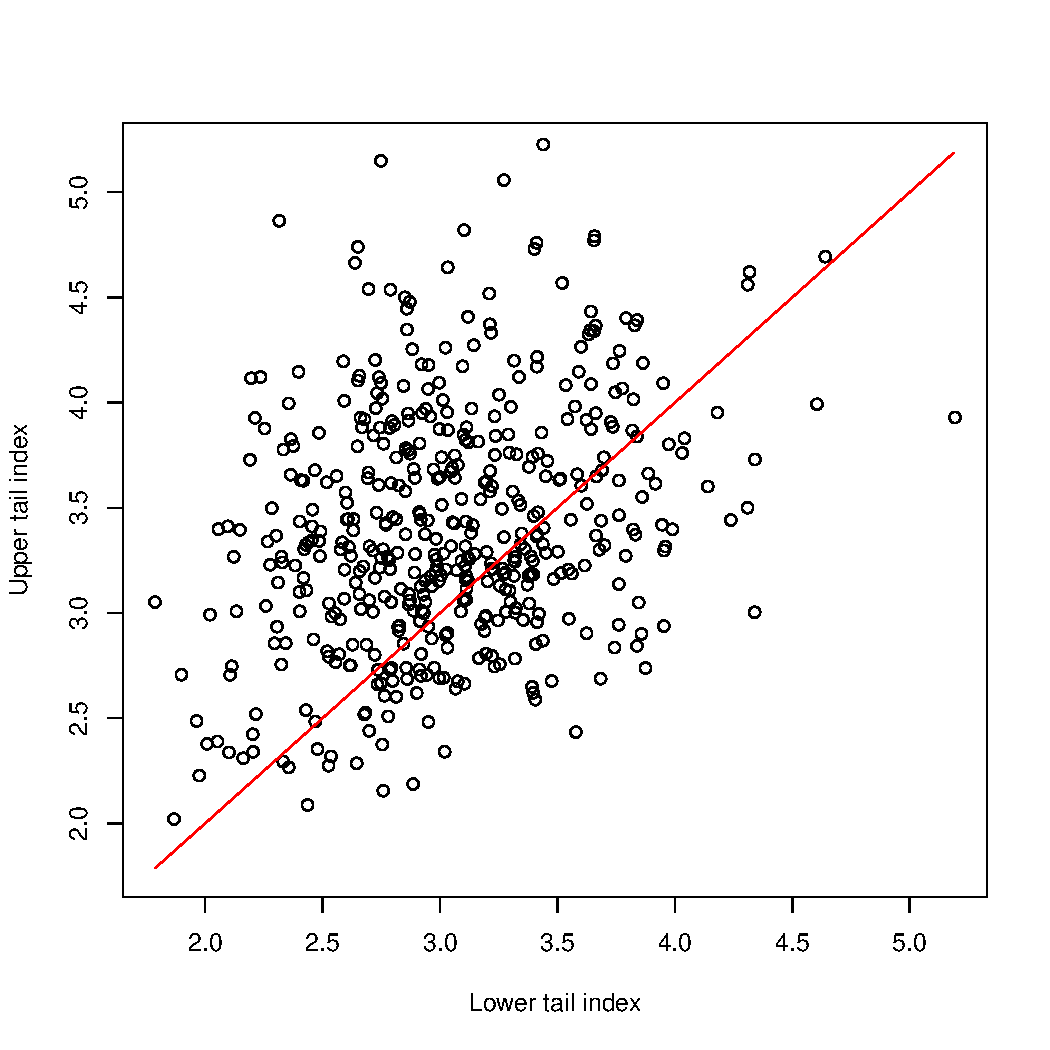
\includegraphics[scale=0.5]{SP500_tail_indices.pdf}
  \caption{Tail indices of stocks included in the S\&P 500 index. The tail
    indices are obtained as their Hill estimators. The red line is the
    line with equal lower- and upper tail indices.}
  \label{fig:SP500_tail_indices}
\end{figure}
It is clear that a large number of stocks have a tail index smaller
than 4, implying a possibly divergent 4th moment. Thus it is of great
importance to study situations where the atomic distribution is
heavy-tailed. This is the topic of the current paper. In particular,
we look into sample covariance matrices with an atomic distribution
that has regularly varying tails.

\newpage
Figure \ref{fig:LamYao} compares the largest eigenvalue of the sum of
time-lagged covariance matrices with the sum of the largest
eigenvalues of individual time-lagged covariance matrices. The data
are return series of 478 stocks selected from the S\&P 500 index.
\begin{figure}[htb!]
  \centering
  \subfigure[] {
    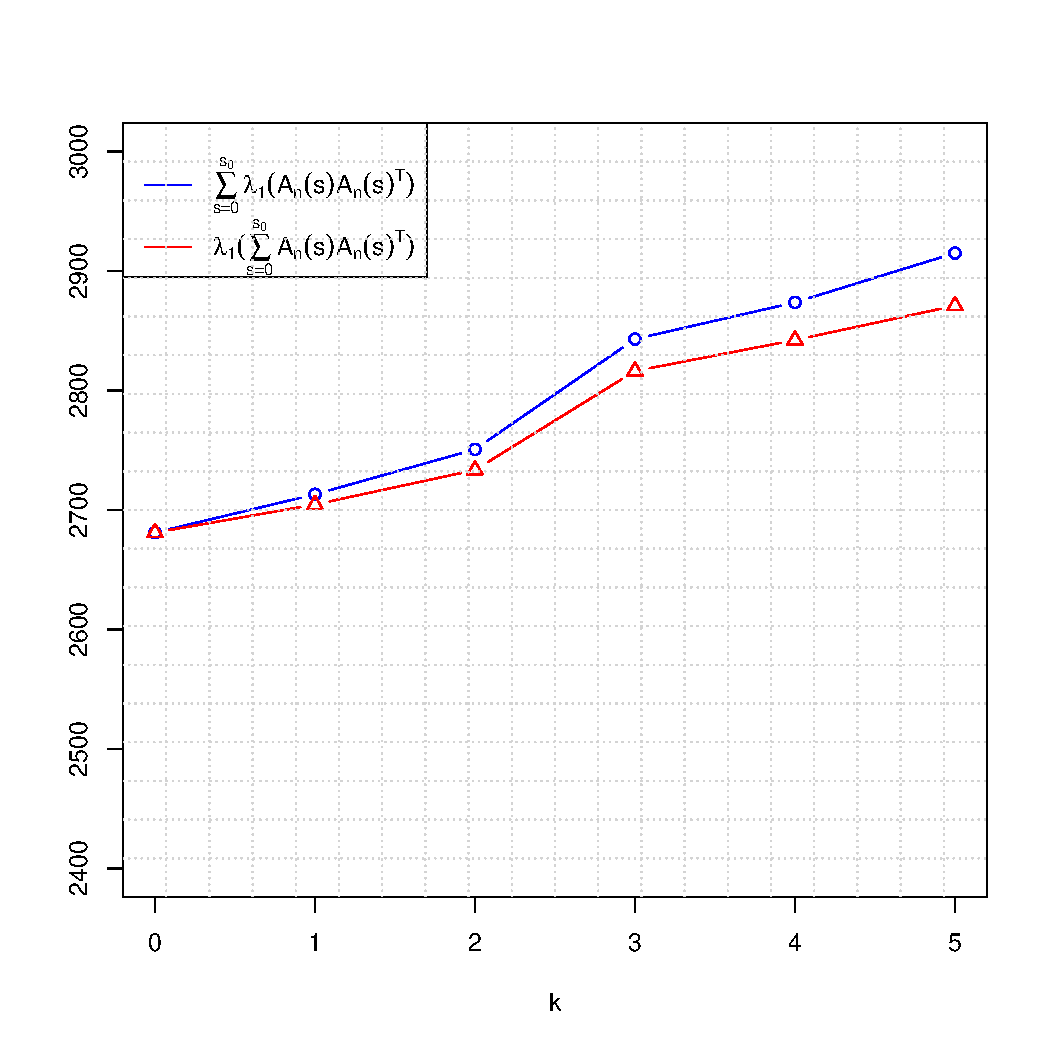
\includegraphics[scale=0.4]{eigen_sum.pdf}
    \label{fig:LamYao:a}
  }
  \subfigure[] {
    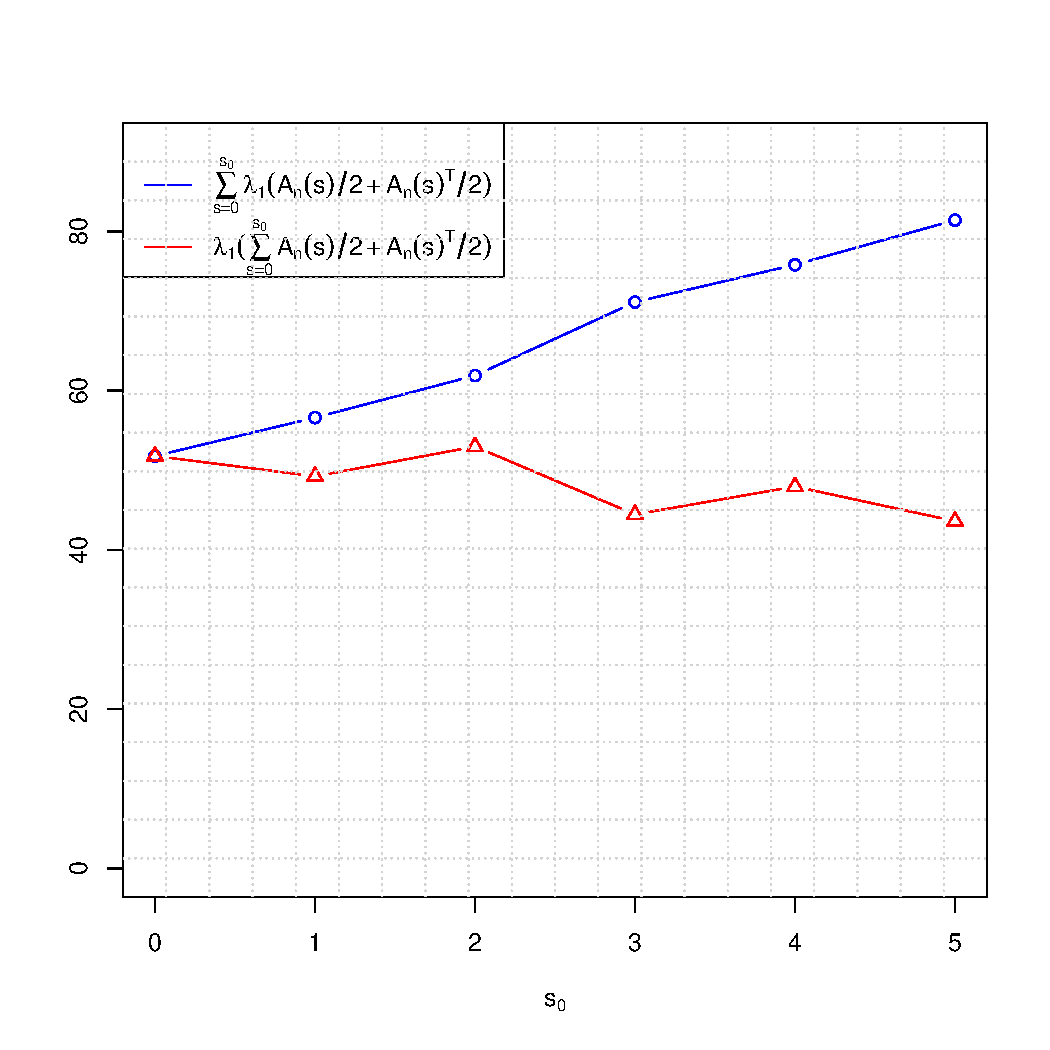
\includegraphics[scale=0.4]{eigen_sum_plus.pdf}
    \label{fig:LamYao:b}
  }
  \caption{The largest eigenvalue of summed time-lagged covariance
    matrices and the sum of the largest eigenvalues of time-lagged
    covariance matrices. In both cases $(C_i)_{lm} =
    \sum_{t=1}^{n-i} X_{lt} X_{m,t+i}$.}
  \label{fig:LamYao}
\end{figure}

\newpage

\subsection{Overview of light-tailed
  case}\label{sec:light_tail_review}
As early as in 1962, T. W. Anderson \cite{anderson:1963} showed that,
when the entries of the data matrix has normal distribution ($\E
X_{ij} = 0$ for $i,j = 1,2,\dots, p$; $\E X_{ii}^2 = 2\sigma^2, \E
X_{ij}^2 = \sigma^2$ for $i \neq j$), the joint density function
of the eigenvalues of the sample covariance matrix is given by
\[
f(\lambda_1, \lambda_2, \dots, \lambda_p; \sigma, p) \propto \prod_{i=1}^p \exp\left(
  -{\lambda_i^2 \over 4\sigma^2}
\right) \prod_{i < j} (\lambda_i - \lambda_j)
\]
In 1988, Yin, Bai and Krishnaiah proved in
\cite{yin:bai:Krishnaiah:1988} the following result for a $p \times n$
matrix $\bf X$ with iid entries $X_{ij}$ under the assumption $\E
X_{11} = 0$, $\E X_{11}^4 < \infty$, and $q = \lim_{n \to \infty} p/n
> 0$
\[
\lambda_{\M}\left({1 \over n}\bf{XX'}\right) \overset{\as}{\to} \left(
  1 + \sqrt{q}
\right)^2 \E X_{11}^2 \text{ as }n \to \infty
\]
When $\E X_{11}^4 = \infty$, Yin and Silverstein proved in 1988
\cite{yin:silverstein:1988}
\[
\lim_{n \to \infty} \sup \lambda_{\M}\left({1 \over
    n}\bf{XX'}\right) = \infty
\]
Later in 2001, I. M. Johnstone showed that, when the data matrix has
standard normal distribution, i.e. $X_{ij} \sim N(0, 1)$, the largest
eigenvalue of the sample covariance matrix follows the Tracy-Widom
distribution:
\[
{ł_1 - \mu_{np} \over \sigma_{np}} \overset{d}{\to} W_1 \sim F_1
\text{ as }{n, p \to \infty}
\]
where $\mu_{np}$ and $\sigma_{np}$ are constants dependent on $p$ and
$n$ and the distribution function $F_1$ is given by
\[
F_1(s) = \exp\left\{
  -{1 \over 2} \int_{s}^\infty \left[
    q(x) + (x - s) q^2(x)
  \right] dx
\right\}
\]
where $q(x)$ is the unique solution to the Painlev\'e II differential
equation
\begin{eqnarray*}
  q''(x) &=& xq(x) + 2 q^3(x) \\
  q(x) &\sim& \text{Ai}(x) \text{ as } x \to \infty
\end{eqnarray*}
Figure \ref{fig:normal-3point-TW} compares the density function of the largest
eigenvalue from simulated $N(0,1)$ and 3-point samples with
that of the Tracy-Widom.
\begin{figure}[htb!]
  \centering
  \subfigure[$N(0, 1)$ entries]{
    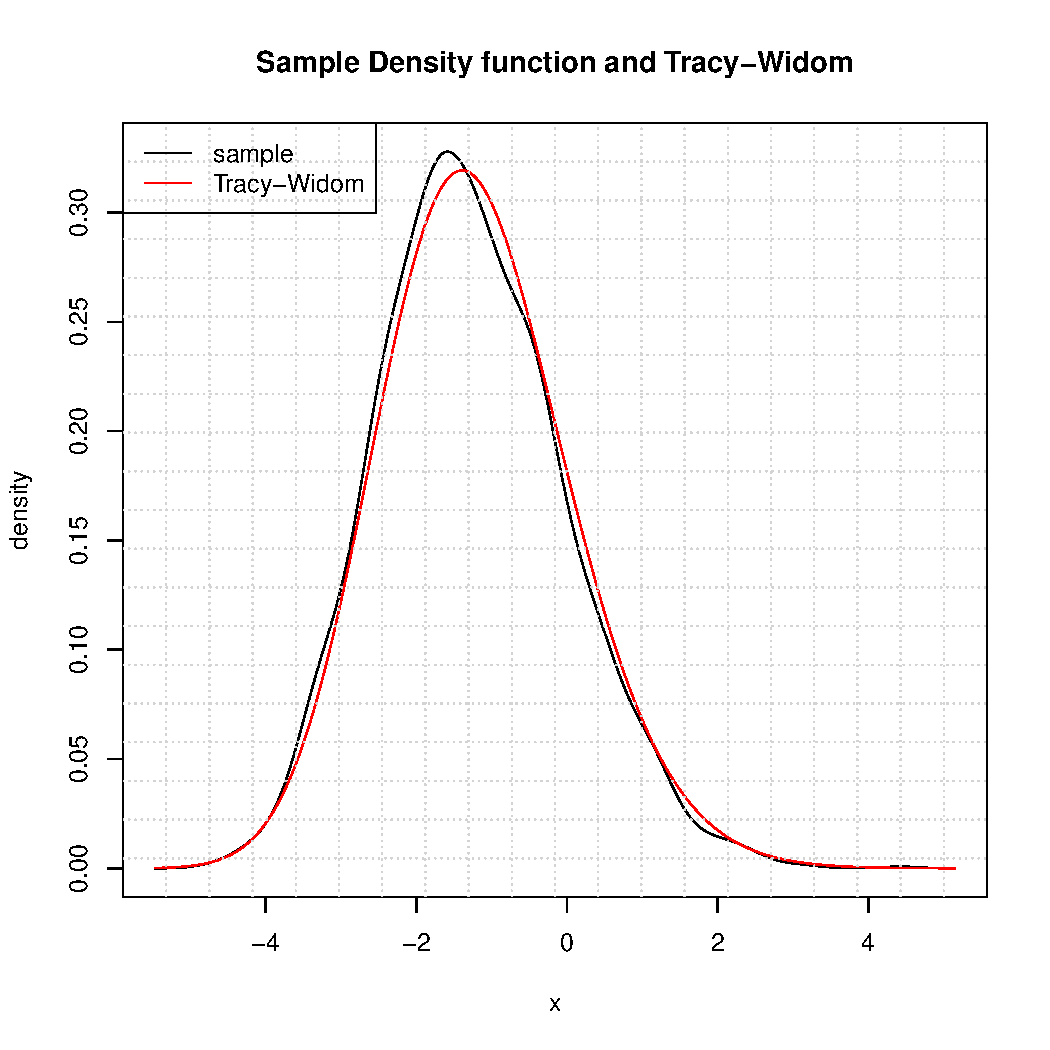
\includegraphics[scale=0.4]{normal-TW.pdf}
  }
  \subfigure[Entry distribution: $\P(X=\sqrt 3) = \P(X=-\sqrt 3 ) =
  1/6$, $\P(X=0)=2/3$. Note $\E X = 0$, $\E X^2 = 1$, $\E X^3 = 0$ and
  $\E X^4 = 3$, i.e. the first 4 moments match those of $N(0, 1).$]{
    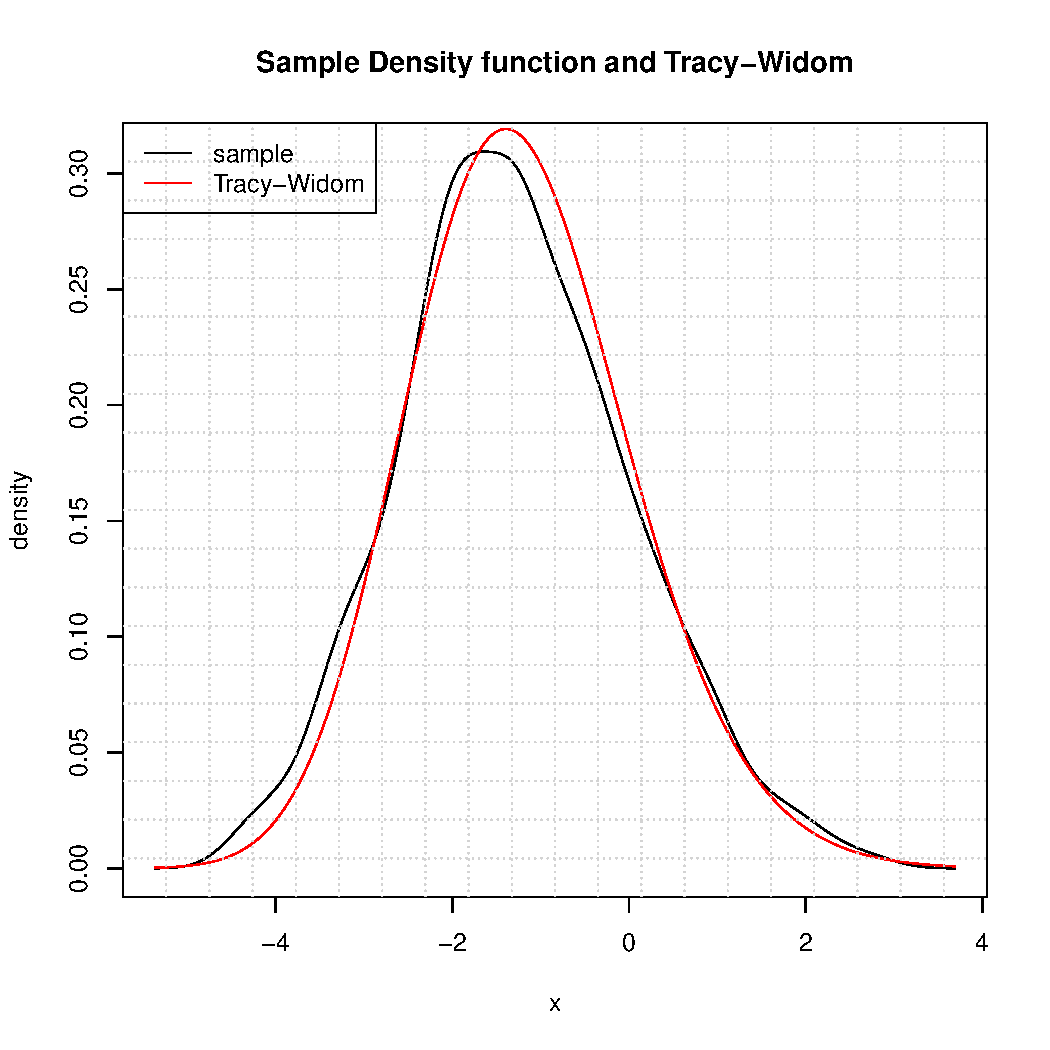
\includegraphics[scale=0.4]{3point-TW.pdf}
  }
  \caption{Sample density function of the largest eigenvalue compared
    with the Tracy-Widom density function. The data matrix has
    dimension $200 \times 1000$. An ensemble of 2000 matrices are
    simulated.}
  \label{fig:normal-3point-TW}
\end{figure}

\newpage
In the case of entry distributions with infinite 4th moment, the
Tracy-Widom law no longer applies and gives way to the Frechet
distribution. Figure \ref{fig:MyDist-Frechet} illustrates this with a
simulated ensemble whose entries are distributed according to
\eqref{eq:mydist} with $\alpha = 1.6$.
\begin{figure}[htb!]
  \centering
  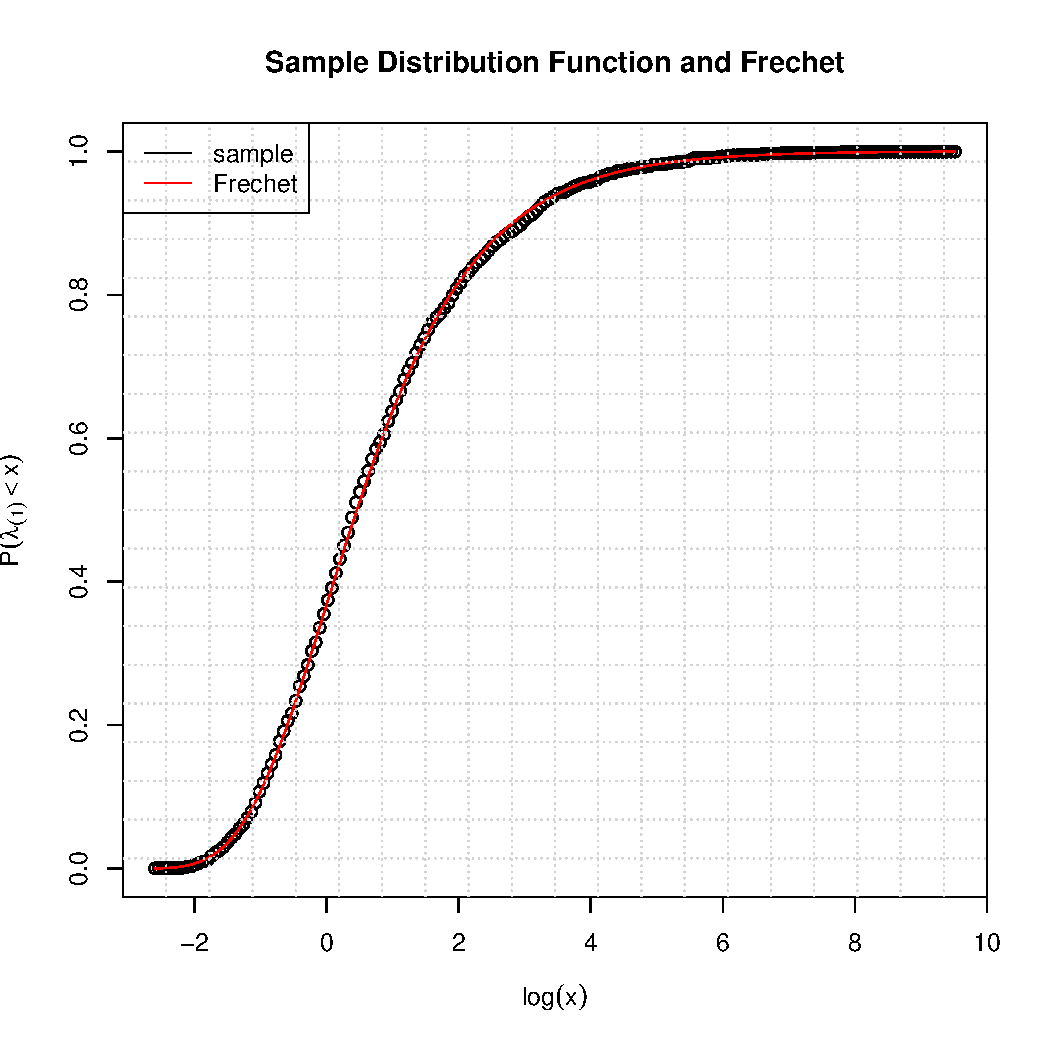
\includegraphics[scale=0.5]{MyDist-Frechet.pdf}  
  \caption{Sample distribution function of the largest eigenvalue
    compared with that of Frechet. The data matrices have dimensions
    $200 \times 1000$. An ensemble of 2000 matrices are simulated.}
  \label{fig:MyDist-Frechet}
\end{figure}

\newpage
Later on, several authors \cite{Pillai:Yin:2011, tao:vu:2012,
  Wang:2012} looked into sample covariance matrix $S_{n, p} = {1
  \over n} \bf{XX}'$, where the entries of $\bf X$, denoted $X_{ij}$
are independent and satisfy the following condition which is referred
to as condition {\bf C0}.
\begin{enumerate}
\item $\E X_{ij} = 0$, $\E X_{ij}^2 = 1$ and
\item $\forall u > 1, \exists \theta > 0$ such that
  \[
  \P(X_{ij} > u) = \theta^{-1} e^{-u^{\theta}}
  \]
\end{enumerate}
Under condition {\bf C0}, Pillai and Yin \cite{Pillai:Yin:2011} proved
that, for $q = \lim_{n \to \infty} {p \over n} \in (0, \infty)
\setminus \{1\}$, the probability of the $j$-th largest eigenvalue of
the sample covariance matrix deviating significantly from its
theoretical value computed as the $1 - j/p$ quantile of the
Marcenko-Pastur distribution decreases exponentially\footnotemark.

\footnotetext{
In precise terms, this means $\forall \zeta > 0, \exists C > 0,
\exists \delta > 0$,
\[
\P\left[
  \left|
    \lambda_{(j)}(S_{n,p}) - \gamma_{j}^{n, p}
  \right| > \varphi^{C} p^{-2/3} \tilde{j}^{-1/3}
\right] \leq p^{\delta} \exp(-\varphi^\zeta)
\]
where $\lambda_{(j)}(S_{n,p})$ is the $j$-th largest eigenvalue of
$S_{n,p}$ and
\begin{eqnarray*}
  \varphi &=& (\log p)^{\log \log p} \\
  \tilde j &=& \min\{(p \wedge n) + 1 - j, j\} \\
  \gamma_{j}^{n, p} &=& \text{inf}\left\{\gamma: \int_\gamma^{\lambda_\M}
  \mu_{n,p}(x) dx \leq {j \over p}\right\} \\
  \lambda_\M &=& (1 + \sqrt q)^2 \\
  \lambda_\m &=& (1 - \sqrt q)^2 \\
  \mu_{n,p}(x) &=& {1 \over 2\pi q x} \sqrt{(x - \lambda_\m)(\lambda_\M - x)}
\end{eqnarray*}
}

Tao and Vu \cite{tao:vu:2012} relaxed the exponential decay condition
of {\bf C0} and replaced it with a high-moment condition, and proved the
four-moment theorem, which was later extended by Wang
\cite{Wang:2012}. In their setting, a $p \times n$ matrix $\bf X$ is
said to obey condition {\bf C1} with constant $c_0$ if $\forall 1
\leq i \leq p, \forall 1 \leq j \leq n$, $\E X_{ij} = 0$, $\E
X_{ij}^2 = 1 $ and $\sup_{i,j} \E|X_{ij}|^{c_0} < C$ for some constant
$C$ independent of $p$ and $n$.

Assume matrices $\bf X$ and $\bf Y$ both satisfy condition {\bf C1}
with constant $c_0$ and in addition they match up to order $4$,
i.e. for all $m, l \geq 0$ such that $m + l \leq 4$, $\E[\mathscr{
R}(X_{ij})^m \mathscr{I}(X_{ij})^l] = \E[\mathscr{R}(Y_{ij})^m
\mathscr{I}(Y_{ij})^l]$ for all $1 \leq i,j \leq p$. Assume also
$\lim_{n \to \infty} p/n = q \in (0, 1]$. Let $G: \mathbb R^k \to
\mathbb R$ be a smooth function obeying the derivative bounds
\[
\left| \nabla^j G(\vec x) \right| < n^{c_0}
\]
for some $c_0 > 0$ and for all $\vec x \in \mathbb R^k$ and all $0
\leq j \leq 5$. Then the following holds for all $1 \leq i_1 \leq i_2
\leq \cdots \leq i_{k} \leq p$, $1 \leq k \leq p$:
\[
\left|
\E G(\lambda_{i_1}, \dots, \lambda_{i_k}) - 
\E G(\omega_{i_1}, \dots, \omega_{i_k})
\right| < n^{- c_0}
\]
where $\lambda_1 \leq \lambda_2, \leq \cdots \leq \lambda_p$ are the
eigenvalues of $\bf XX'$ and $\omega_1 \leq \omega_2, \leq
\cdots \leq \omega_p$ are those of $\bf YY'$.

Moreover, even when ${\bf XX'}$ and ${\bf YY'}$ only match to order
3, the above inequality still holds provided that the bounds on the
derivatives are strengthened to
\[
|\nabla^j G(\vec x)| < n^{-j c_1}
\]
for all $0 \leq j \leq 5$, all $\vec x \in \mathbb R^k$ and some $c_1$
that is sufficiently large compared to $c_0$.

%------------------------------------------------------------------------
\section{The iid heavy-tailed case}

\subsection{\texorpdfstring{$\alpha \in (0,2)$}{alpha in (0,2)}:
  Overview of existing results: Davis et al., Soshnikov, Auffiner et
  al.}
\subsection{\texorpdfstring{$\alpha \in (0,2)$}{alpha in (0,2)}: Our
  extension of these results; only order statistics of \texorpdfstring{$Z_{it}$}{Z[it]}'s
  necessary and no sums (proof by the technical result)}
To illustrate the validity of the results, we pick the following
distribution function for $Z$ and compare the eigenvalues with
the order statistics of $D_i = \sum_{t=1}^n Z_{it}^2$ and $Z^2$ using
simulated data.
\begin{equation}
  \label{eq:mydist}
  f(x) = {d \over dx}\P(Z \leq x) = \left\{
    \begin{array}{ll}
      {\alpha \over (4|x|)^{\alpha + 1}} & |x| > 1/4 \\
      \alpha & \text{ otherwise }
    \end{array}
  \right.
\end{equation}
This function is shown in figure \ref{fig:densitySim}.
\begin{figure}[htb!]
  \centering
  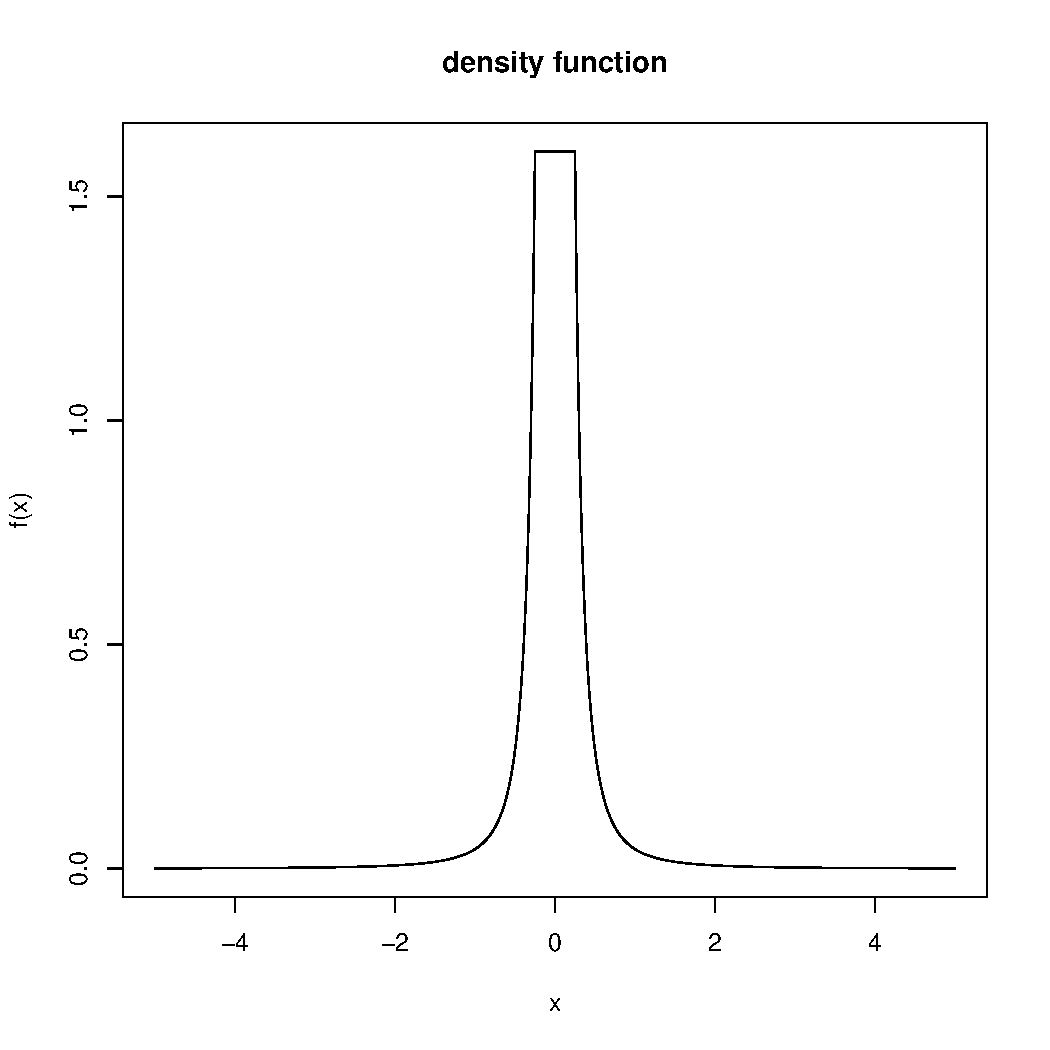
\includegraphics[scale=0.40]{densitySim.pdf}
  \caption{Density function of simulated data. $\alpha=1.6$ is chosen
    for simulation.}
  \label{fig:densitySim}
\end{figure}
Using the simulated data, empirical density functions are obtained for
$a_{np}^{-2}\lambda_{(i)} - a_{np}^{-2}D_{(i)}$ and
$a_{np}^{-2}\lambda_{(i)} - a_{np}^{-2}Z^2_{(i)}$. These are shown in
figure \ref{fig:lambda_comparison}.
\begin{figure}[htb!]
  \centering
  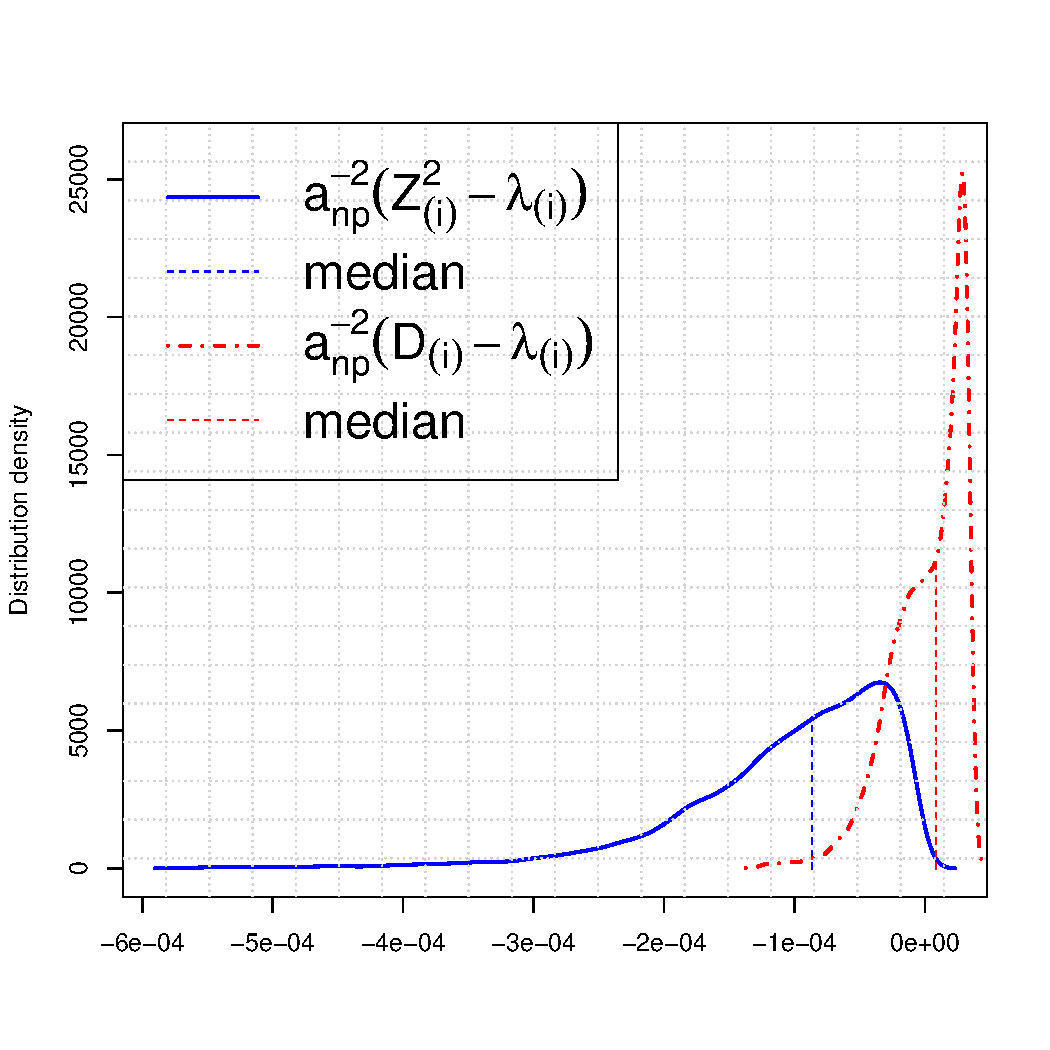
\includegraphics[scale=0.40]{lambda_comparison.pdf}
  \caption{A total of 20000 pairs are compared in each case.}
  \label{fig:lambda_comparison}
\end{figure}




\subsection{\texorpdfstring{$\alpha \in [2,4)$}{alpha in [2,4)}: Overview of existing results: Davis et
  al., Soshnikov, Auffiner et al.}
\subsection{\texorpdfstring{$\alpha \in [2,4)$}{alpha in [2,4)}: The problem of centering and restrictions on \texorpdfstring{$p_n$}{p[n]}}
\subsection{\texorpdfstring{$\alpha \in [2,10/3)$}{alpha in [2,10/3)}: Our new result for the UN-CENTERED
  sample covariance matrix; only order statistics of \texorpdfstring{\texorpdfstring{$Z_{it}$}{Z[it]}}{Z[it]}'s
  necessary and no sums (proof by the technical result)}
\subsection{\texorpdfstring{$\alpha \in [10/3,4)$}{alpha in [10/3,4)}: A conjecture with partial proof for
  the UN-CENTERED sample covariance matrix)}

%------------------------------------------------------------------------
\section{Extension to linear dependence, two-sided filters}

\subsection{\texorpdfstring{$\alpha \in (0,10/3)$}{alpha in (0,10/3)}: Eigenvalues of the sample covariance matrix}
\subsection{\texorpdfstring{$\alpha \in [10/3,4)$}{alpha in [10/3,4)}: Eigenvalues of the CENTERED sample covariance matrix}
\subsection{\texorpdfstring{$\alpha \in [2,4)$}{alpha in [2,4)} and
  \texorpdfstring{$p/n \to \gamma \in (0,1]$}{p/n tends to gamma in (0,1]}:
  Eigenvalues of the sample covariance matrix using Auffinger's
  result}
\subsection{Point process convergence}

%------------------------------------------------------------------------
\section{Applications of the results in the previous section}

\subsection{Ratio of second to largest eigenvalue (to power become uniform), self-normalizing sums, ratio of largest eigenvalue to trace, simulations, figures,...}
\subsection{Functions acting on the eigenvalues}
\subsection{Figures: Ratios of consecutive eigenvalues, illustrations for financial data, ...}
\subsection{S\&P data using ranks}
For real financial data, it is unreasonable to expect all
the time series under consideration to have the same tail index. So a
procedure of standardization has to be adopted. In this section we
use the rank transform.

Suppose we have $p$ time series each of length $n$ and have arranged
them in a $p\times n$ matrix $R_{it}$, where $i = 1, 2, \dots, p$ and
$t=1,2, \dots, n$. For each row of $X$, we transform it as
\begin{eqnarray*}
  X_{it} &=& -\left[
    \log \left({1 \over n+1} \sum_{\tau=1}^n \1_{R_{i\tau} \leq R_{it}} \right)
  \right]^{-1}
\end{eqnarray*}
When $R_{i1}, R_{i2}, \dots, R_{in}$ are iid for each $i$, the
argument to the $\log$ function is asymptotically uniformly
distributed as $n \to \infty$, and hence $X_{it}$ is a standard
Fr\'echet r.v.

Figure \ref{fig:EigenRatio} shows the ratio of successive eigenvalues
of the matrix $a_{np}^{-2}XX'$, where the rows of matrix $X$ comprise
the rank-transformed sequences of a number of selected time series
in the S\&P 500 index.
\begin{figure}[htb!]
  \centering
  \subfigure[]{
    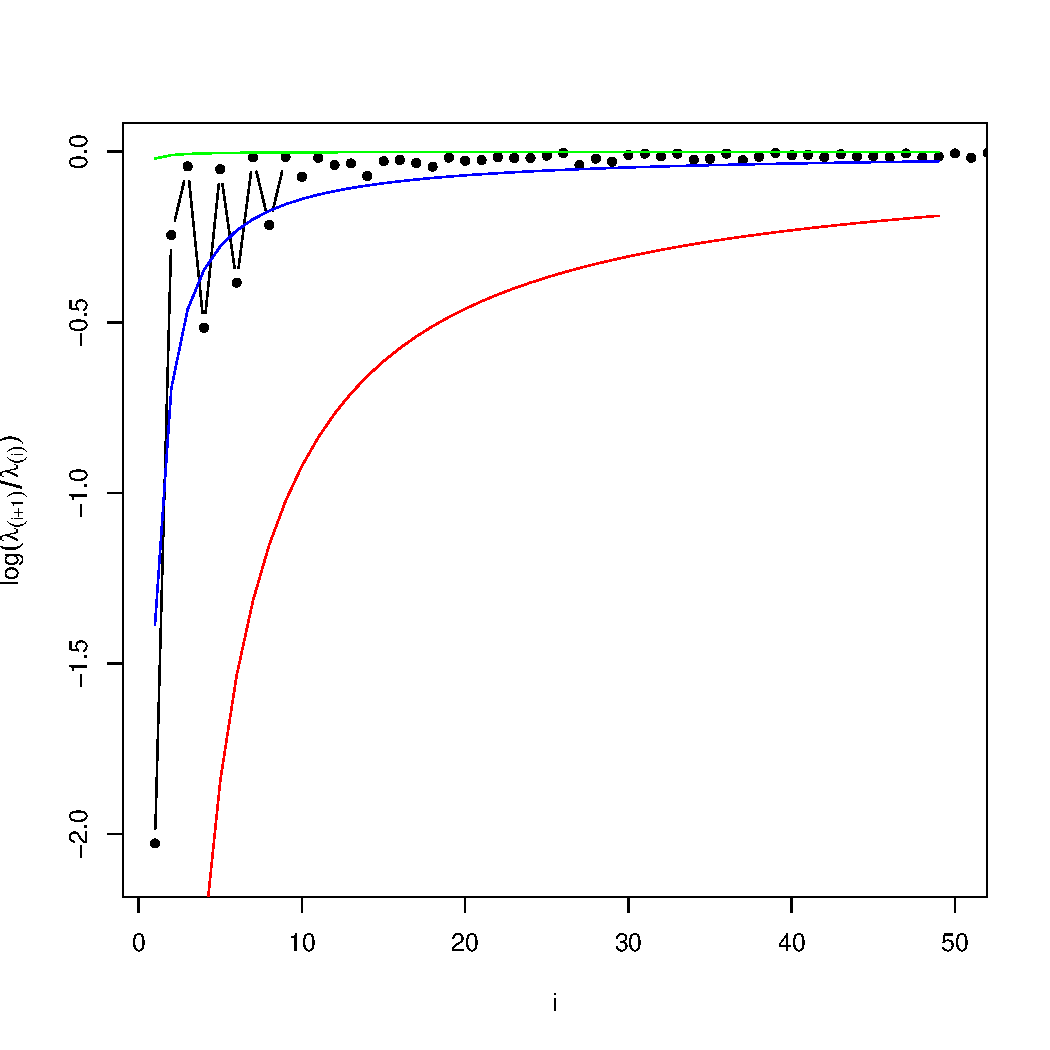
\includegraphics[scale=0.40]{EigenRatioSP500_50_shown.pdf}
  }
  \subfigure[]{
    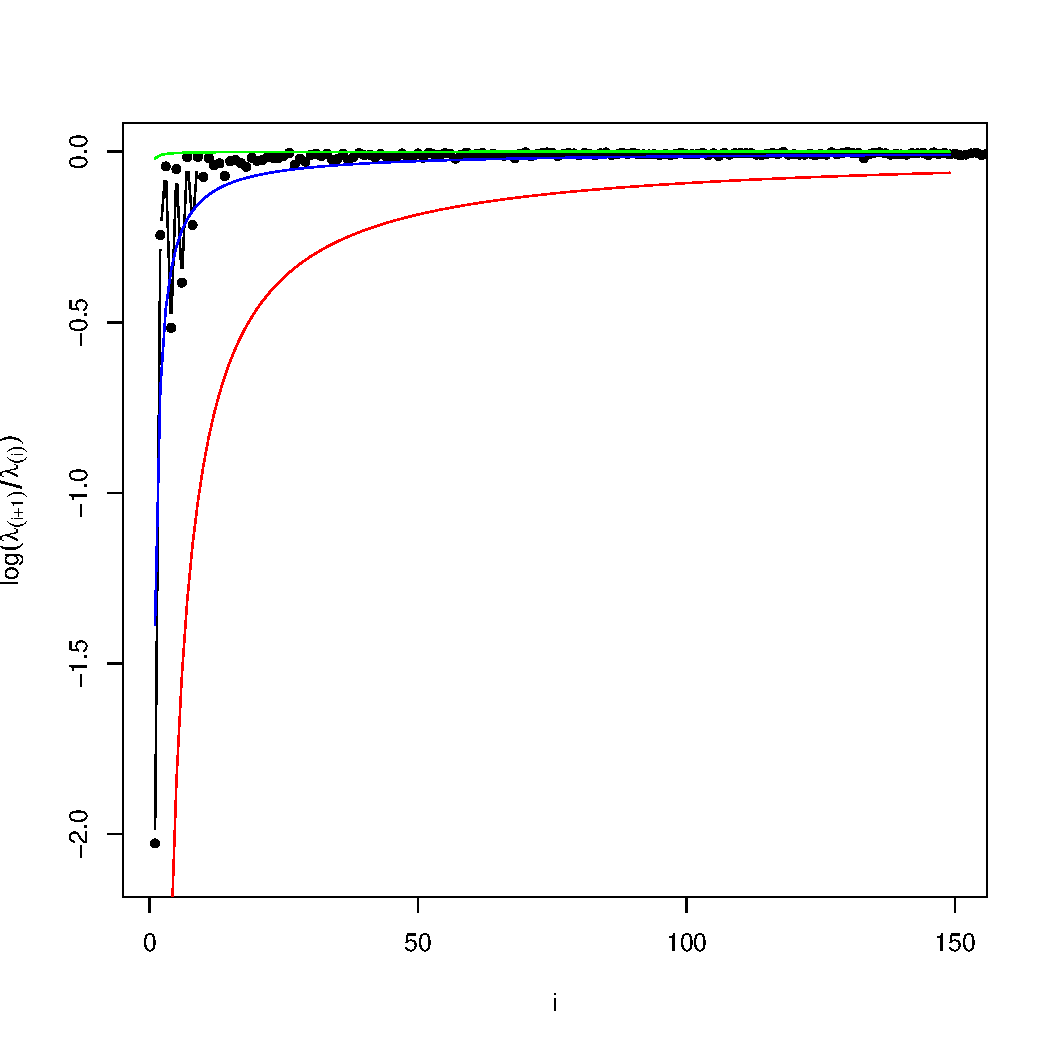
\includegraphics[scale=0.40]{EigenRatioSP500_150_shown.pdf}
  }
  \subfigure[]{
    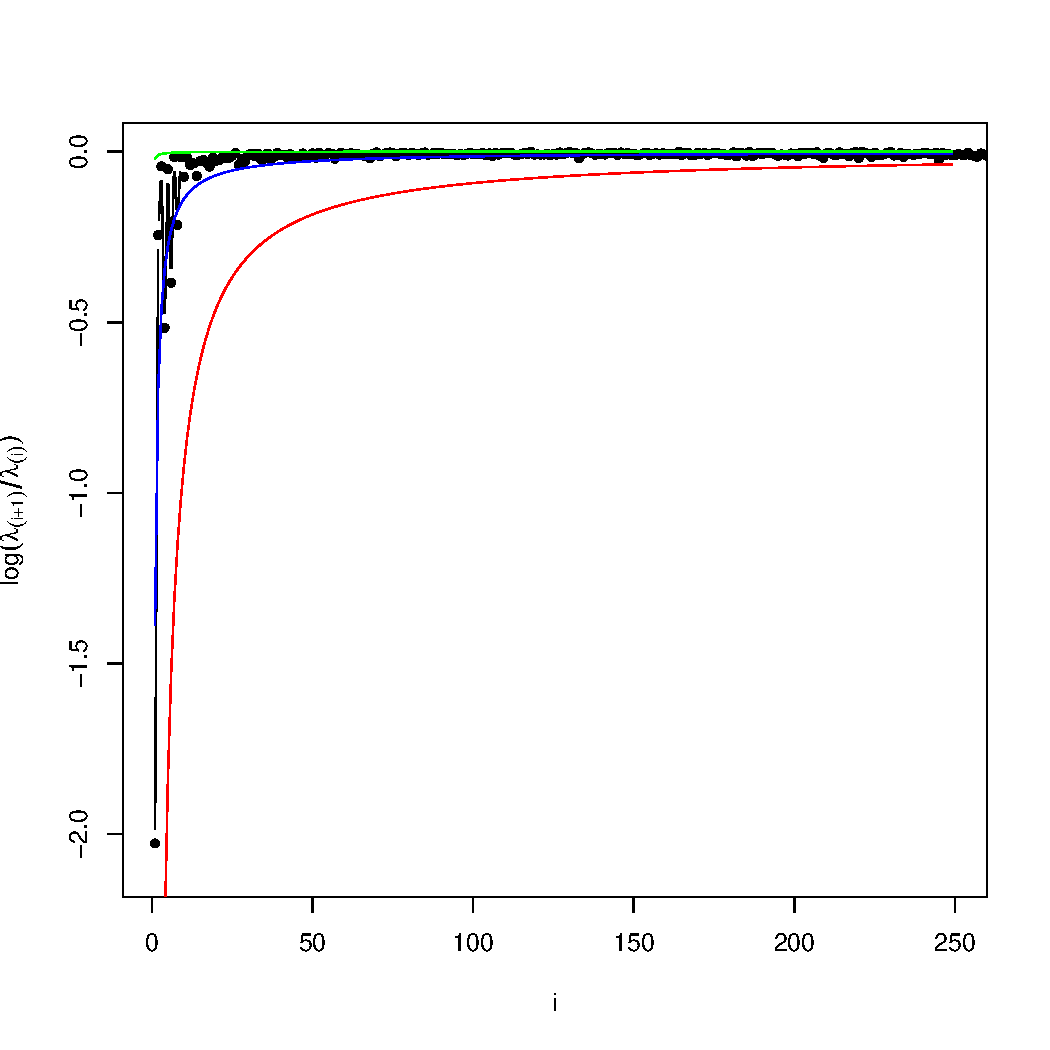
\includegraphics[scale=0.40]{EigenRatioSP500_250_shown.pdf}
  }
  \subfigure[]{
    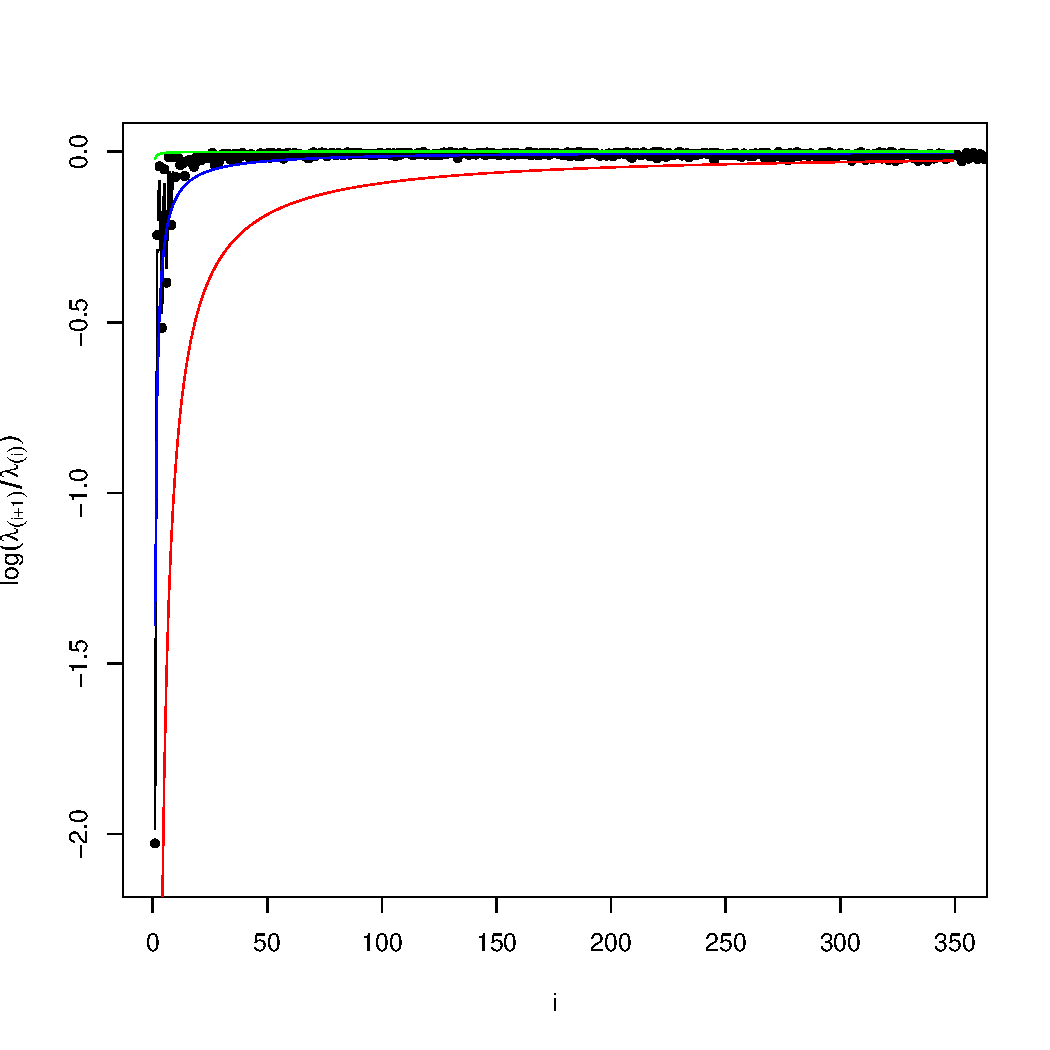
\includegraphics[scale=0.40]{EigenRatioSP500_350_shown.pdf}
  }
  \caption{$\lambda_{(i+1)} / \lambda_{(i)}$ versus $i$, The blue line
  is the median of the ratio, the red line is the 1\% quantile
  and the green line is the 99\% quantile.}
  \label{fig:EigenRatio}
\end{figure}
It is seen that, as $i \to \infty$, $\lambda_{(i+1)} / \lambda_{(i)}
\to 1$. This is in fact expected based on the theory explained in the
previous sections. Suppose the coefficients $h_{kl}$ is separable,
i.e. $h_{kl} = \theta_k c_l$, then, as shown in previous sections,
\[
\sum_{i=1}^p \pp{a_{np}^{-2}\lambda_{(i)}} \overset{d}{\to}
\sum_{i=1}^\infty \pp{\Gamma_i^{-2} \lambda_H}
\]
where $\lambda_H$ is the solo non-zero eigenvalue of $\bf H$. Note
that the tail index $\alpha=1$ for the ranks. So it is clear
\[
{\lambda_{(i+1)} \over 
  \lambda_{(i)}} \overset{d}{=} \left({\Gamma_i \over
    \Gamma_{i+1}}\right)^{2}=\left(1 - {E_{i+1} \over E_1 + E_2
    + \dots E_{i+1}}\right)^{2} \to 1 \text{ as } i \to \infty
\]
where $E_k, k=1,2,\dots,i+1$ are iid. exponential rv. In fact the
distribution function of $\lambda_{(i+1)} / \lambda_{(i)}$ is rather
simple. Recall
\[
{\Gamma_{i} \over \Gamma_{i+1}} \overset{d}{=} U_{1, i}
\]
where $U_{1, i}$ is the largest upper order statistic of a
$\text{Uniform}(0, 1)$ sample of size $i$. So
\begin{eqnarray*}
\P\left[{\lambda_{(i+1)} \over \lambda_{(i)}} \leq x \right] &=& x^{i/2}
%\E \left[{\lambda_{(i+1)} \over \lambda_{(i)}} \right] &=& {i \over i + 2}
\end{eqnarray*}
The median and confident intervals marked in figure
\ref{fig:EigenRatio} are calculated according to the above formulas.

\subsection{Probability Mass Due To Correlations}
In figure \ref{fig:ProbMass} the distribution function of
${\lambda_{(1)} - \lambda_{(2)} \over \lambda_{(1)}}$ in the cases of
iid data and correlated data, which are described in {\color{red} fill
in here}, is illuatrated. The predicted probability mass at 3/4 is
clearly seen.
\begin{figure}[htb!]
  \centering
  \subfigure[iid data]{
    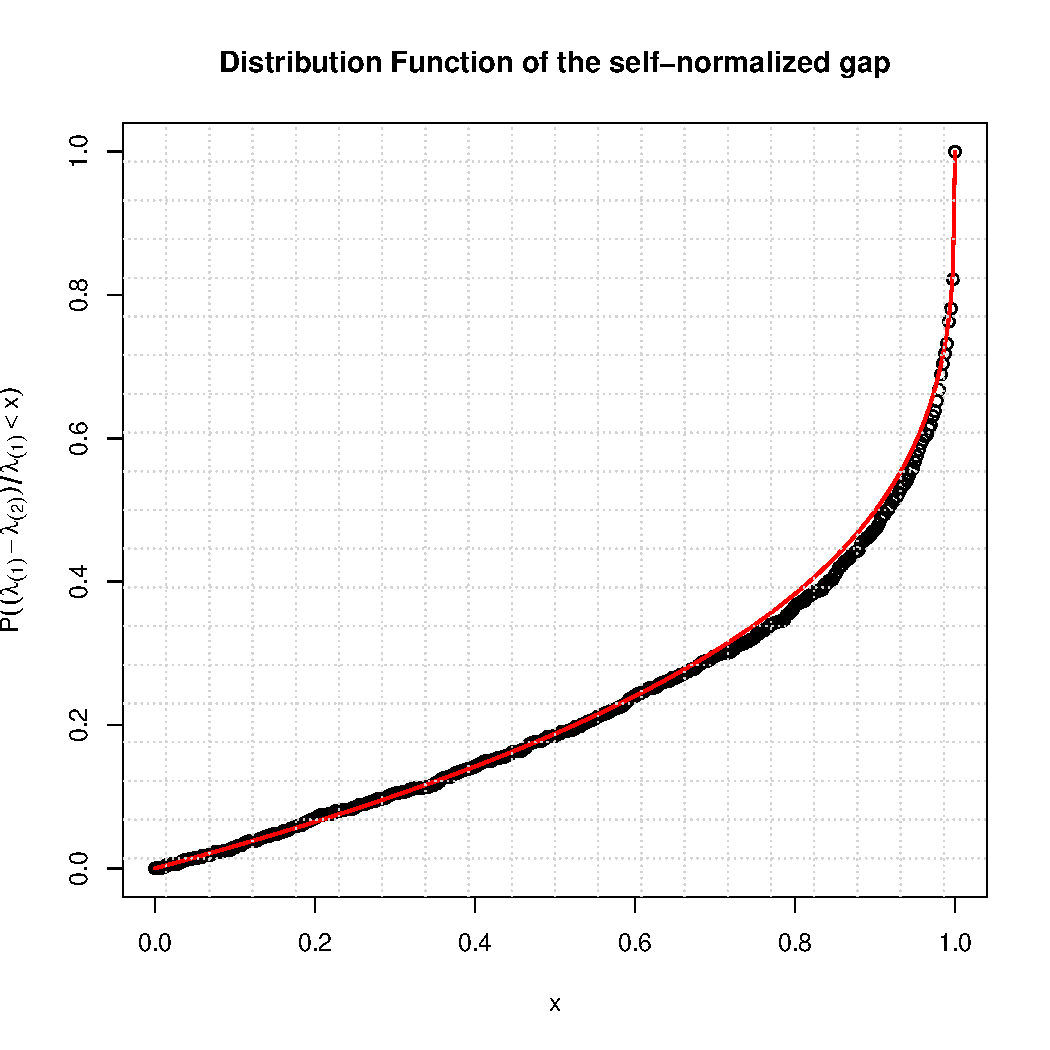
\includegraphics[scale=0.4]{lambda_1_2_Gaps_iid.pdf}
  }
  \subfigure[Correlated data]{
    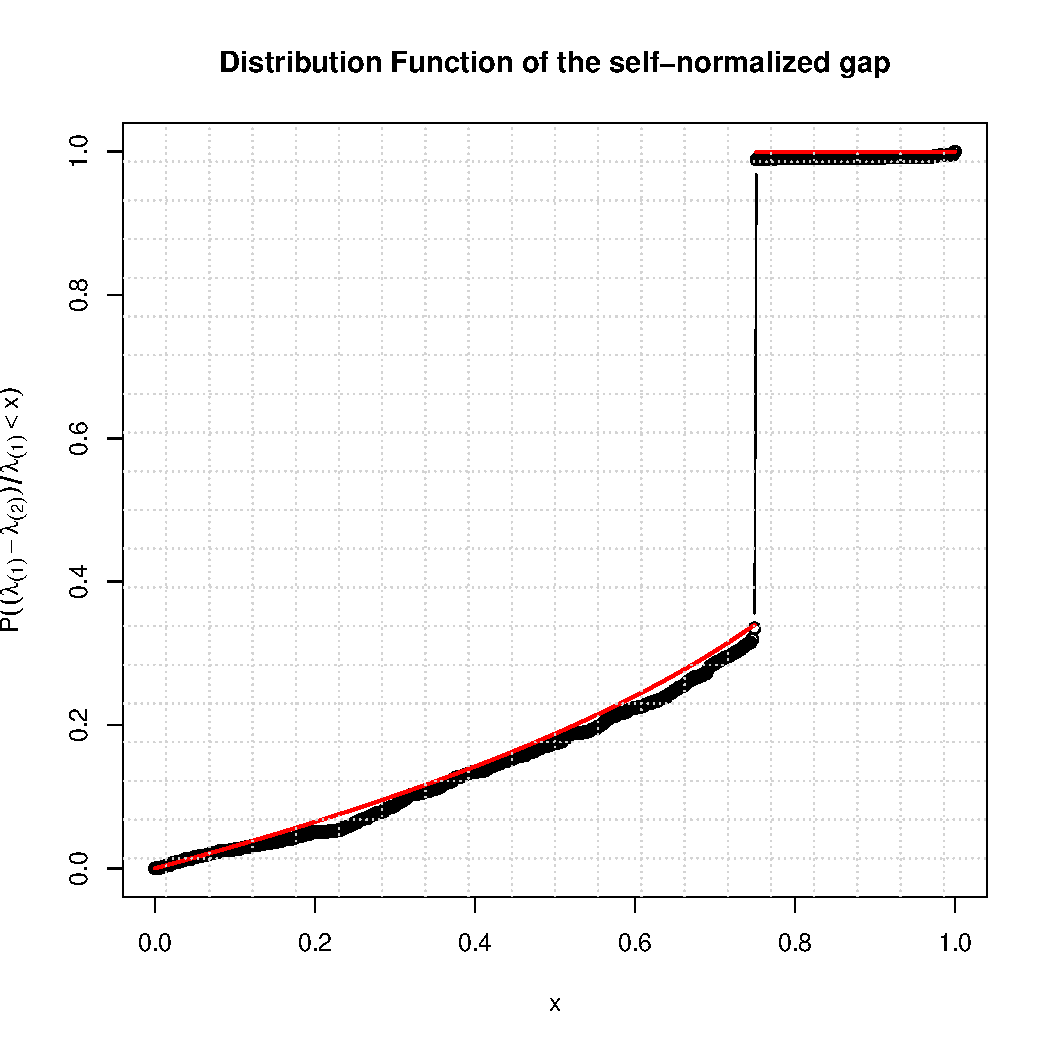
\includegraphics[scale=0.4]{lambda_1_2_Gaps.pdf}
  }
  \caption{Distribution function of ${\lambda_{(1)} - \lambda_{(2)} \over
      \lambda_{(1)}}$ in the cases of iid data and correlated
    data. The data matrices have dimension $200 \times 1000$. 1000
    data matrices are simulated in each case. The data have the
    distribution described in \eqref{eq:mydist} with $\alpha=0.6$.}
  \label{fig:ProbMass}
\end{figure}

%------------------------------------------------------------------------
\section{A further extension: The sample autocovariance function}

\subsection{\texorpdfstring{$\alpha \in (0,10/3)$}{alpha in (0,10/3)}: Eigenvalues of the sample
  autocovariance matrix}
\subsection{\texorpdfstring{$\alpha \in [10/3,4)$}{alpha in [10/3,4)}: Eigenvalues of the CENTERED sample
  autocovariance matrix}

%------------------------------------------------------------------------
\section{Applications of the results for the autocovariance function}

\subsection{Sums of largest eigenvalues vs.~ largest eigenvalues of
  sums, application to real data + plots}
\subsection{Explanation of these plots in the separable case,
  discussion of the two methods to ensure real eigenvalues, link to
  Lam + Yao}

%------------------------------------------------------------------------
\section{Non-linear theory, independent rows + large deviations, SV
  and GARCH, SV with multivariate Gaussian and t-distributed noise}
%------------------------------------------------------------------------
\section{Future directions, discussion of the conjecture}


%------------------------------------------------------------------------
\appendix 
\section{Regular variation, large deviations and point processes}
\section{The key technical result to identify the largest eigenvalues
  with the order statistics of the squares of the matrix entries in
  the iid case}
\section{A lemma which shows that the sample covariance matrix is
  approximated by its diagonal in the iid case (more involved than
  simple matrix norms)}
\section{The Proofs}












%-----------------------------------------------------------------------
%Bibliography
%Bibliography
\begin{thebibliography}{99}
\baselineskip12pt
%AAAAAAAAAAAAAAAAAAAAAAAAAAAAAAAAAAAAAAAAAAAAAAAAAAAAAAAAAAAAAAA
\bibitem{anderson:1963}
{\sc Anderson, T.W.,}\ (1963)
{\em Asymptotic theory for principal component analysis.}  {\em Ann.~Math.~Statist.} {\bf 34}, 122--148.
%\bibitem{anderson:guionnet:zeitouni:2008}
%{\sc Anderson, G.W., Guionnet, A. and Zeitouni, O.}\ (2008)
%{\em An Introduction to Random Matrices.}  Cambridge
%University Press, Cambridge (UK).

\bibitem{auffinger:arous:peche:2009}
{\sc Auffinger, A., Ben Arous, G. and P\'ech\'e, S.}\ (2009)
Poisson convergence for the largest eigenvalues of heavy tailed random
matrices.
{\em Ann. Inst. H. Poincar\'e, Probab. Statist.} {\bf 45}, 589--610.
%BBBBBBBBBBBBBBBBBBBBBBBBBBBBBBBBBBBBBBBBBBBBBBBBBBBBBBBBBBBBBBB
%\bibitem{bai:silverstein:2010}
%{\sc Bai, Z. and Silverstein, J.W.}\ (2010)
%{\em Spectral Analysis of Large Dimensional Random Matrices.} 2nd
%Edition. Springer, New York.
%\bibitem{belinschi:dembo:guionnet:2009}
%{\sc Belinschi, S.,  Dembo, A. and Guionnet, A.}\ (2009)
%Spectral measure of heavy tailed band and covariance random matrices.
%{\em Comm. Math. Phys.}  {\bf 289}, 1023--1055.
%\bibitem{arous:guionnet:2008}
%{\sc  Ben Arous, G. and  Guionnet, A.} \ (2008)
%The spectrum of heavy tailed random matrices.  {\em Comm. Math. Phys.}
%{\bf 278}, 715--751.
\bibitem{bhatia:1997}
{\sc Bhatia, R.}\ (1997)
{\em Matrix Analysis.} Springer, New York.
\bibitem{bingham:goldie:teugels:1987}
{\sc Bingham, N.H., Goldie, C.M.\ and Teugels, J.L.}\ (1987)
{\em Regular Variation.} Cambridge University Press, Cambridge.
%\bibitem{bose:hazra:saha:2009}
%{\sc Bose, A., Subhra Hazra, R. and  Saha, K.}\ (2009)
%Limiting spectral distribution of circulant type matrices
%with dependent inputs.  {\em Electron. J. Probab.}  {\bf 14},
%2463--2491.
%\bibitem{bose:hazra:saha:2010}
%{\sc Bose, A., Subhra Hazra, R. and  Saha, K.}\ (2010)
%Spectral norm of circulant type matrices with heavy tailed entries.
%{\em Electron. Commun. Probab.}  {\bf 15}, 299--313.
%CCCCCCCCCCCCCCCCCCCCCCCCCCCCCCCCCCCCCCCCCCCCCCCCCCCCCCCCCCCCCCC
\bibitem{cline:hsing:1998}
{\sc Cline, D.B.H. and Hsing, T.}\ (1998)
Large deviation probabilities for sums of random variables
with heavy or subexponential tails. Technical report.
Statistics Dept., Texas A\&M University. %Available as \begin{verbatim}http://www.stat.tamu.edu/~dcline/Papers/large5.pdf \end{verbatim}
%DDDDDDDDDDDDDDDDDDDDDDDDDDDDDDDDDDDDDDDDDDDDDDDDDDDDDDDDDDDDDDD
\bibitem{davis:resnick:1985}
{\sc
Davis, R.A. and Resnick, S.I.}\ (1985)
Limit theory for moving averages of random variables
with regularly varying tail probabilities.
{\em Ann. Probab.} {\bf 13}, 179--195.
\bibitem{davis:pfaffel:stelzer:2014}
{\sc Davis, R.A., Pfaffel, O. and Stelzer, R.}\ (2014)
Limit theory for the largest eigenvalues of
sample covariance matrices with heavy tails.
{\em Stoch. Proc. Appl.} {\bf 124}, 18--50.

\bibitem{denisov:dieker:shneer:2008}
{\sc Denisov, D., Dieker, A.B. and Shneer, V.}\ (2008)
Large deviations for random walks under subexponentiality:
the big-jump domain.
{\em Ann. Probab.} {\bf 36}, 1946--1991.

%EEEEEEEEEEEEEEEEEEEEEEEEEEEEEEEEEEEEEEEEEEEEEEEEEEEEEEEEEEEEEEE

\bibitem{embrechts:goldie:1980}
{\sc Embrechts, P. and Goldie,C.}\ (1980)
On closure and factorization theorems for subexponential and related
distributions. {\em J. Austral. Math. Soc.,} Ser. A {\bf 29}, 243--256.

%\bibitem{embrechts:kluppelberg:mikosch:1997}
%{\sc Embrechts, P., Kl\"uppelberg, C. and Mikosch, T.}\ (1997)
%{\em Modelling Extremal Events for Insurance and Finance.}
%Springer,  Berlin.

%GGGGGGGGGGGGGGGGGGGGGGGGGGGGGGGGGGGGGGGGGGGGGGGGGGGGGGGGGGGGGGG

\bibitem{gohberg:goldberg:krupnik:2000}
{\sc Gohberg, I., Goldberg, S. and N. Krupnik}\ (2000)
{\em Traces and Determinants of Linear Operators.} Birkh\"auser, Basel.

\bibitem{johnstone:2001}
{\sc Johnstone, I.M.}\ (2001)
{\em on the distribution of the largest eigenvalue in principal component analysis.} {\em Ann.~Statist.} {\bf 29} (2), 295--327.

%MMMMMMMMMMMMMMMMMMMMMMMMMMMMMMMMMMMMMMMMMMMMMMMMMMMMMMMMMMMMMMM

\bibitem{mikosch:samorodnitsky:2000}
{\sc Mikosch, T. and Samorodnitsky, G.} \ (2000)
The supremum of a negative drift random walk with
dependent heavy-tailed steps. {\em Ann. Appl. Probab.} {\bf 10}, 1025--1064.

%NNNNNNNNNNNNNNNNNNNNNNNNNNNNNNNNNNNNNNNNNNNNNNNNNNNNNNNNNNNNNNN

\bibitem{nagaev:1979}
{\sc Nagaev, S.V.}\ (1979)
Large deviations of sums of independent random
variables.
{\em Ann. Probab.} {\bf 7}, 745--789.

%PPPPPPPPPPPPPPPPPPPPPPPPPPPPPPPPPPPPPPPPPPPPPPPPPPPPPPPPPPPPPPP

\bibitem{petrov:1995}
{\sc Petrov, V.V.} (1995)
{\em Limit Theorems of Probability Theory.} Oxford University Press,
Oxford.

%RRRRRRRRRRRRRRRRRRRRRRRRRRRRRRRRRRRRRRRRRRRRRRRRRRRRRRRRRRRRRRR

\bibitem{resnick:1987}
{\sc Resnick, S.I.}\ (1987)
{\em Extreme Values, Regular Variation, and Point Processes.}
Sprin\-ger, New York.

\bibitem{yin:bai:Krishnaiah:1988}
{\sc Y.Q. Yin and Z.D. Bai and P.R. Krishnaiah}\ (1988)
On the Limit of the Largest Eigenvalue of the Large Dimensional Sample
Covariance Matrix.
{\em Probability Theory and Related Fields} {\bf 78}, 509--521.

\bibitem{yin:silverstein:1988}
{\sc Y.Q. Yin and Jack W. Silverstein}\ (1988)
A Note on the Largest Eigenvalue of a Large Dimensional Sample
Covariance Matrix
{\em Journal of Multivariate Analysis} {\bf 26} (2), 166--168.

\bibitem{resnick:2007}
{\sc Resnick, S.I.}\ (2007)
{\em Heavy-Tail Phenomena: Probabilistic and Statistical Modeling.}
Springer, New York.

%SSSSSSSSSSSSSSSSSSSSSSSSSSSSSSSSSSSSSSSSSSSSSSSSSSSSSSSSSSSSSSS

\bibitem{samorodnitsky:taqqu:1994}
{\sc Samorodnitsky, G. and Taqqu, M.S.}\ (1994)
{\em Stable Non-Gaussian Random Processes.
Stochastic Models with Infinite Variance.} Chapman and Hall, London.

%\bibitem{soshnikov:2004}
%{\sc Soshnikov, A.}\ (2004)
%Poisson statistics for the largest eigenvalues of Wigner matrices with
%heavy tails. {\em Electr. Comm. Probab.} {\bf 9}, 82--91.

\bibitem{soshnikov:2006}
{\sc Soshnikov, A.}\ (2006)
Poisson statistics for the largest eigenvalues in random matrix
ensembles.
In: {\em Mathematical Physics of Quantum Mechanics.} Lecture Notes in
Physics {\bf 690}. Springer, Berlin, pp. 351--364.

\bibitem{Pillai:Yin:2011}
{\sc N. Pillai and J. Yin}\ (2011)
Universality of covariance matrices
{\em arXiv:1110.2501,2011}

\bibitem{tao:vu:2012}
{\sc Tao, T. and Vu, V.}\ (2012)
Random covariance matrices; universality of local statistics of eigenvalues.
{\em Ann.~Probab.} {\bf 40} (3), 1285--1315.

%K. Wang. Random covariance matrices: universality of local statistics of
%eigenvalues up to the edge. RMTA, 1(1), 2012.
\bibitem{Wang:2012}
{\sc K. Wang}\ (2012)
Random covariance matrices: universality of local statistics of
eigenvalues up to the edge
{\em RMTA} {\bf 1} (1)

\end{thebibliography}
\end{document}
